% =====================================================================
%  ROS2 Multithreaded Simulation Architecture -- TikZ figures
%  Self-contained: compile with pdflatex to preview both figures.
%  To reuse in asme_paper.tex, copy whichever \begin{tikzpicture}...\end{tikzpicture}
%  block into a figure/figure* environment (the tikz libraries below must be
%  loaded in the main preamble).
% =====================================================================
\documentclass[11pt]{article}

\usepackage[margin=1.5cm]{geometry}
\usepackage{tikz}
\usepackage{amsmath}
\usetikzlibrary{positioning,shapes.geometric,arrows.meta,fit,backgrounds,calc}

% ---------- shared styles ----------
\tikzset{
  % generic process box
  proc/.style    = {rectangle, rounded corners=2pt, draw=black!70, thick,
                    fill=blue!6, align=center, inner sep=4pt,
                    minimum height=8mm, font=\small},
  % start/end terminator
  term/.style    = {ellipse, draw=black!70, thick, fill=violet!18,
                    align=center, inner sep=3pt, minimum height=8mm, font=\small\bfseries},
  % decision diamond
  dec/.style     = {diamond, aspect=2.2, draw=black!70, thick, fill=orange!18,
                    align=center, inner sep=1pt, font=\footnotesize},
  % FSM state pill
  state/.style   = {rectangle, rounded corners=6pt, draw=teal!80!black, thick,
                    fill=teal!10, align=center, inner sep=3pt,
                    minimum height=7mm, minimum width=24mm, font=\small},
  % publisher / subscriber I/O box
  io/.style      = {rectangle, draw=black!60, fill=green!8, align=center,
                    font=\scriptsize, inner sep=3pt, minimum height=6mm},
  % external / hardware-sim layer
  ext/.style     = {rectangle, rounded corners=2pt, draw=black!70, thick,
                    fill=gray!12, align=center, font=\small, inner sep=4pt,
                    minimum height=9mm},
  % lane background
  lane/.style    = {rectangle, rounded corners=4pt, draw=blue!30, dashed,
                    fill=blue!3, inner sep=6pt},
  % arrows
  flow/.style    = {-{Stealth[length=2.4mm]}, thick, black!75},
  bus/.style     = {{Stealth[length=2.2mm]}-{Stealth[length=2.2mm]}, thick, black!65},
}

\begin{document}

% =====================================================================
%  FIGURE A -- Concurrent execution architecture (the "system" view)
%  Emphasises: one node -> MultiThreadedExecutor -> N independent
%  callback groups running in parallel -> DDS bridge -> PX4/Gazebo.
% =====================================================================
\begin{center}
{\large\bfseries Figure A: Concurrent ROS2--PX4 Simulation Architecture}\\[4pt]
\end{center}

\begin{center}
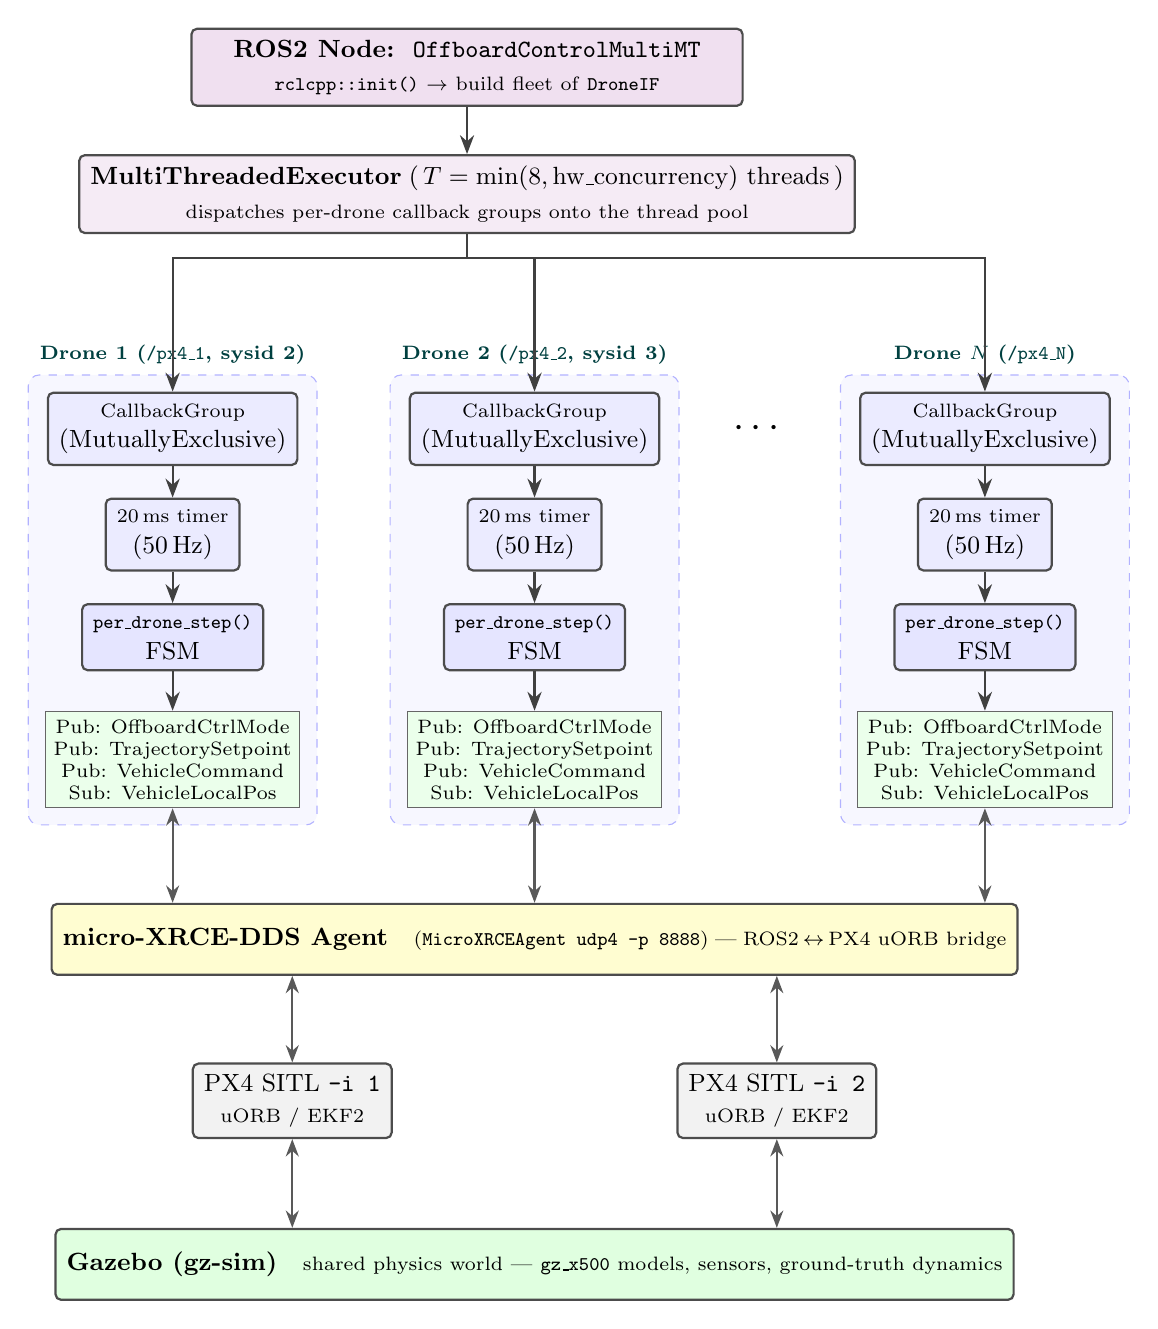
\begin{tikzpicture}[node distance=6mm and 10mm]

  % --- top: node + executor ---
  \node[proc, fill=violet!12, minimum width=70mm] (node)
       {\textbf{ROS2 Node:}\; \texttt{OffboardControlMultiMT}\\[1pt]
        \scriptsize \texttt{rclcpp::init()} $\rightarrow$ build fleet of \texttt{DroneIF}};

  \node[proc, below=of node, minimum width=70mm, fill=violet!8] (exec)
       {\textbf{MultiThreadedExecutor}\;(\,$T=\min(8,\text{hw\_concurrency})$ threads\,)\\[1pt]
        \scriptsize dispatches per-drone callback groups onto the thread pool};

  \draw[flow] (node) -- (exec);

  % --- three parallel drone lanes ---
  % each lane: callback group -> 20ms timer -> per_drone_step() -> I/O
  \def\laneY{-30mm}

  % --- lane content macro-style (manual for control) ---
  % Lane 1 (extra vertical gap below the executor so the lane labels don't crowd it)
  \node[proc, anchor=north, fill=blue!8] (cg1) at ($(exec.south west)+(12mm,-20mm)$)
       {\scriptsize CallbackGroup\\(MutuallyExclusive)};
  \node[proc, below=4mm of cg1, fill=blue!8] (t1)
       {\scriptsize 20\,ms timer\\(50\,Hz)};
  \node[proc, below=4mm of t1, fill=blue!10] (s1)
       {\scriptsize \texttt{per\_drone\_step()}\\ FSM};
  \node[io, below=5mm of s1] (io1)
       {Pub: OffboardCtrlMode\\Pub: TrajectorySetpoint\\Pub: VehicleCommand\\Sub: VehicleLocalPos};

  % Lane 2
  \node[proc, right=14mm of cg1, fill=blue!8] (cg2)
       {\scriptsize CallbackGroup\\(MutuallyExclusive)};
  \node[proc, below=4mm of cg2, fill=blue!8] (t2)
       {\scriptsize 20\,ms timer\\(50\,Hz)};
  \node[proc, below=4mm of t2, fill=blue!10] (s2)
       {\scriptsize \texttt{per\_drone\_step()}\\ FSM};
  \node[io, below=5mm of s2] (io2)
       {Pub: OffboardCtrlMode\\Pub: TrajectorySetpoint\\Pub: VehicleCommand\\Sub: VehicleLocalPos};

  % Lane N (dots + template)
  \node[right=8mm of cg2, font=\Large\bfseries] (dots) {$\cdots$};
  \node[proc, right=8mm of dots, fill=blue!8] (cgN)
       {\scriptsize CallbackGroup\\(MutuallyExclusive)};
  \node[proc, below=4mm of cgN, fill=blue!8] (tN)
       {\scriptsize 20\,ms timer\\(50\,Hz)};
  \node[proc, below=4mm of tN, fill=blue!10] (sN)
       {\scriptsize \texttt{per\_drone\_step()}\\ FSM};
  \node[io, below=5mm of sN] (ioN)
       {Pub: OffboardCtrlMode\\Pub: TrajectorySetpoint\\Pub: VehicleCommand\\Sub: VehicleLocalPos};

  \draw[flow] (cg1) -- (t1); \draw[flow] (t1) -- (s1); \draw[flow] (s1) -- (io1);
  \draw[flow] (cg2) -- (t2); \draw[flow] (t2) -- (s2); \draw[flow] (s2) -- (io2);
  \draw[flow] (cgN) -- (tN); \draw[flow] (tN) -- (sN); \draw[flow] (sN) -- (ioN);

  % executor -> each callback group
  \draw[flow] (exec.south) -- ++(0,-3mm) -| (cg1);
  \draw[flow] (exec.south) -- ++(0,-3mm) -| (cg2);
  \draw[flow] (exec.south) -- ++(0,-3mm) -| (cgN);

  % lane backgrounds (drawn behind)
  \begin{scope}[on background layer]
    \node[lane, fit=(cg1)(io1), label={[font=\scriptsize\bfseries,teal!50!black]above:Drone 1 (\texttt{/px4\_1}, sysid 2)}] {};
    \node[lane, fit=(cg2)(io2), label={[font=\scriptsize\bfseries,teal!50!black]above:Drone 2 (\texttt{/px4\_2}, sysid 3)}] {};
    \node[lane, fit=(cgN)(ioN), label={[font=\scriptsize\bfseries,teal!50!black]above:Drone $N$ (\texttt{/px4\_N})}] {};
  \end{scope}

  % --- DDS bus ---
  \node[ext, fill=yellow!18, below=12mm of io2, minimum width=120mm] (dds)
       {\textbf{micro-XRCE-DDS Agent}\quad\scriptsize(\texttt{MicroXRCEAgent udp4 -p 8888})\;---\;ROS2\,$\leftrightarrow$\,PX4 uORB bridge};

  \draw[bus] (io1) -- (io1|-dds.north);
  \draw[bus] (io2) -- (dds.north);
  \draw[bus] (ioN) -- (ioN|-dds.north);

  % --- PX4 SITL instances (sit just below the DDS bus) ---
  \node[ext, below left=11mm and 18mm of dds.south, fill=gray!10] (px1)
       {PX4 SITL \texttt{-i 1}\\\scriptsize uORB / EKF2};
  \node[ext, below right=11mm and 18mm of dds.south, fill=gray!10] (px2)
       {PX4 SITL \texttt{-i 2}\\\scriptsize uORB / EKF2};

  \draw[bus] (px1.north) -- (px1.north|-dds.south);
  \draw[bus] (px2.north) -- (px2.north|-dds.south);

  % --- Gazebo (clears the PX4 row: 32mm below the DDS bus) ---
  \node[ext, below=32mm of dds, fill=green!12, minimum width=120mm] (gz)
       {\textbf{Gazebo (gz-sim)}\quad\scriptsize shared physics world ---
        \texttt{gz\_x500} models, sensors, ground-truth dynamics};

  \draw[bus] (px1.south) -- (px1.south|-gz.north);
  \draw[bus] (px2.south) -- (px2.south|-gz.north);

\end{tikzpicture}
\end{center}

\vspace{1.2cm}

% =====================================================================
%  FIGURE B -- Per-drone FSM executed every 20 ms timer tick
%  This replaces the old linear flowchart and shows the feedback loop.
% =====================================================================
\begin{center}
{\large\bfseries Figure B: Per-Drone Finite-State Machine (20\,ms Timer Callback)}\\[4pt]
\end{center}

\begin{center}
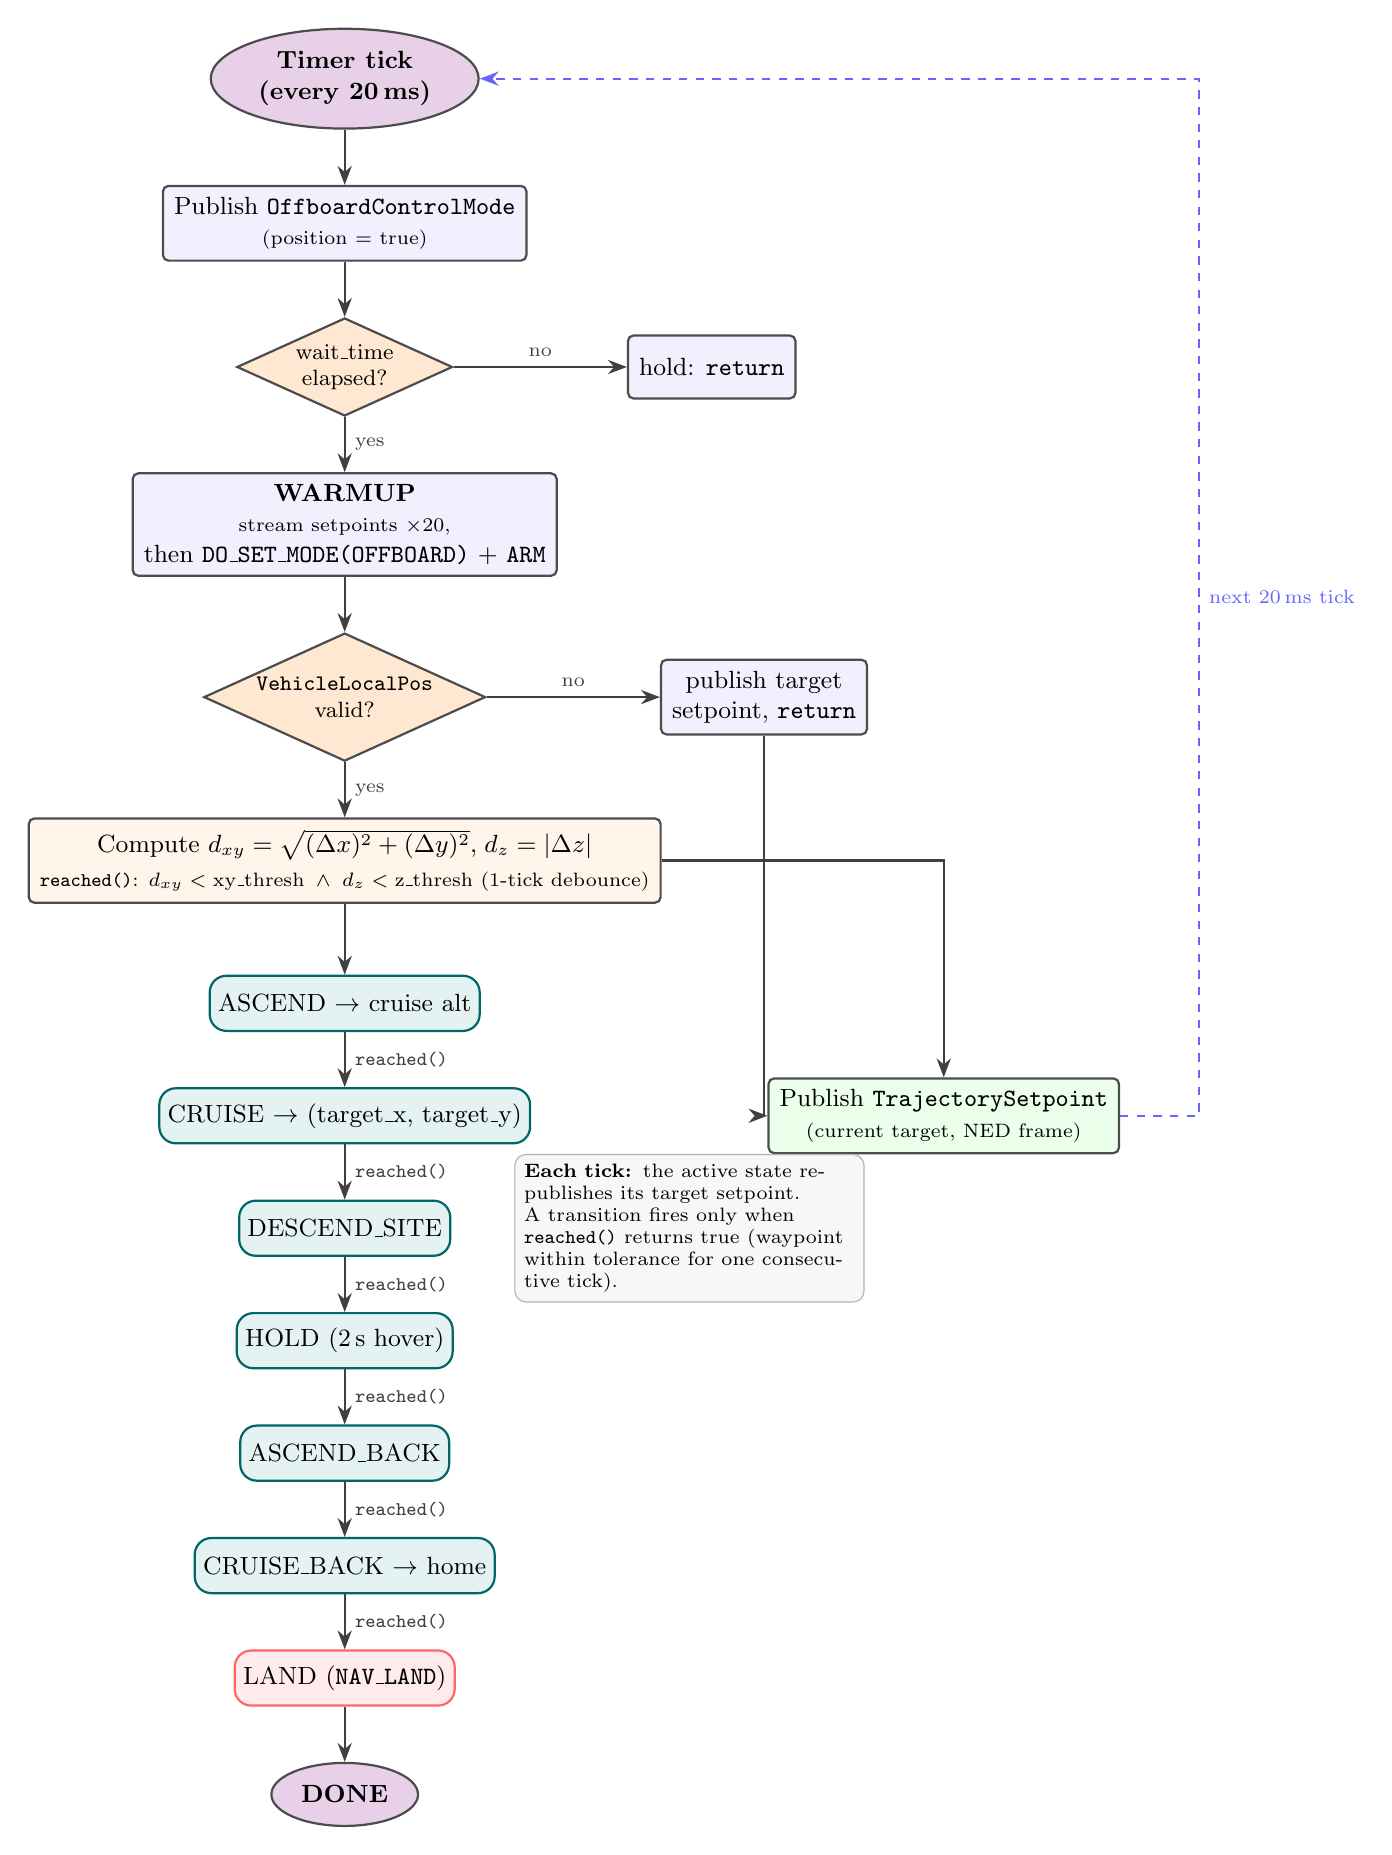
\begin{tikzpicture}[node distance=7mm and 14mm]

  \node[term] (tick) {Timer tick\\(every 20\,ms)};

  \node[proc, below=of tick] (ofb)
       {Publish \texttt{OffboardControlMode}\\\scriptsize(position = true)};

  \node[dec, below=of ofb] (waited)
       {wait\_time\\elapsed?};

  \node[proc, right=22mm of waited] (hold0)
       {hold: \texttt{return}};

  \node[proc, below=of waited] (warm)
       {\textbf{WARMUP}\\\scriptsize stream setpoints $\times 20$,\\ then \texttt{DO\_SET\_MODE(OFFBOARD)} + \texttt{ARM}};

  \node[dec, below=of warm] (posval)
       {\texttt{VehicleLocalPos}\\valid?};

  \node[proc, right=22mm of posval] (hold1)
       {publish target\\setpoint, \texttt{return}};

  % FSM core: compute distances + reached()
  \node[proc, below=of posval, fill=orange!8] (dist)
       {Compute $d_{xy}=\sqrt{(\Delta x)^2+(\Delta y)^2}$,\;$d_z=|\Delta z|$\\[1pt]
        \scriptsize \texttt{reached()}: $d_{xy}<\text{xy\_thresh}\;\wedge\;d_z<\text{z\_thresh}$ (1-tick debounce)};

  % the state ladder
  \node[state, below=9mm of dist] (sasc)   {ASCEND $\rightarrow$ cruise alt};
  \node[state, below=of sasc]     (scru)   {CRUISE $\rightarrow$ (target\_x, target\_y)};
  \node[state, below=of scru]     (sdes)   {DESCEND\_SITE};
  \node[state, below=of sdes]     (shold)  {HOLD (2\,s hover)};
  \node[state, below=of shold]    (sascb)  {ASCEND\_BACK};
  \node[state, below=of sascb]    (scrub)  {CRUISE\_BACK $\rightarrow$ home};
  \node[state, below=of scrub, fill=red!8, draw=red!60] (sland) {LAND (\texttt{NAV\_LAND})};

  \node[term, below=of sland] (done) {DONE};

  % publish setpoint (loop tail)
  \node[proc, right=30mm of scru, fill=green!8] (pubsp)
       {Publish \texttt{TrajectorySetpoint}\\\scriptsize (current target, NED frame)};

  % --- edges ---
  \draw[flow] (tick) -- (ofb);
  \draw[flow] (ofb) -- (waited);
  \draw[flow] (waited) -- node[above,font=\scriptsize]{no} (hold0);
  \draw[flow] (waited) -- node[right,font=\scriptsize]{yes} (warm);
  \draw[flow] (warm) -- (posval);
  \draw[flow] (posval) -- node[above,font=\scriptsize]{no} (hold1);
  \draw[flow] (posval) -- node[right,font=\scriptsize]{yes} (dist);
  \draw[flow] (dist) -- (sasc);

  % state ladder advances on reached()
  \foreach \a/\b in {sasc/scru, scru/sdes, sdes/shold, shold/sascb, sascb/scrub, scrub/sland} {
    \draw[flow] (\a) -- node[right,font=\scriptsize]{\texttt{reached()}} (\b);
  }
  \draw[flow] (sland) -- (done);

  % every branch publishes a setpoint then waits for next tick
  \draw[flow] (dist.east) -| (pubsp);
  \draw[flow] (hold1) |- (pubsp);

  % loop-back: next tick (dashed feedback)
  \draw[flow, dashed, blue!60] (pubsp.east) -- ++(10mm,0)
        |- node[pos=0.25,right,font=\scriptsize,blue!60]{next 20\,ms tick} (tick.east);

  % "stay in current state if not reached" self-explainer
  \node[font=\scriptsize, align=left, draw=black!30, fill=black!3, rounded corners,
        right=8mm of sdes, text width=42mm] (note)
       {\textbf{Each tick:} the active state re-publishes its target setpoint.
        A transition fires only when \texttt{reached()} returns true
        (waypoint within tolerance for one consecutive tick).};

\end{tikzpicture}
\end{center}

\end{document}
